% docs/texte/20_core/signal.tex -- chapter "Signal Simulation" (Interferosim)
% Version: 0.2.0 (2026-11-01) -- section "Baseband and quantisation" (interferosim 0.9.2)
%   0.1.0 (2026-10-31): package interferosim.signal (interferosim 0.4.0)
% ================================================================
\label{ch:signal}
\index{signal simulation}\index{IQ samples}

The package \texttt{interferosim.signal} generates the complex baseband
samples (IQ) that the SDR of every station records, from a sky model
(chapter~\ref{ch:sky-models}), an array (chapter~\ref{ch:array}) and a
receiver profile (chapter~\ref{ch:receiver}). It closes the simulation
chain at the level of the measured data: the correlator, imaging and
deconvolution can be tested on simulated recordings exactly as on real
ones. Origin: AAS6 \texttt{modules/sdr/iq\_record\_node.py}
(\texttt{\_SimDualSource}) and \texttt{modules/interfero/skysim.py},
extended to several sources, any number of stations and instrument errors.
Notebook: \texttt{03\_signal\_simulation.ipynb}.

\section{Signal model}

A source of flux density $S$ radiates a stationary complex Gaussian signal
$s(t)$ of power $S$. Station $k$ receives it delayed by $\tau_k(t)$ relative
to the reference station; mixing with the LO at $f_c$ to complex baseband
adds the phase $-2\pi f_c\tau_k$:
\begin{equation}
  x_k(t) = \sum_c \sqrt{P_k(\theta_c)}\; s_c\bigl(t-\tau_k(t)\bigr)\,
           e^{-2\pi i f_c\tau_k(t)} + n_k(t)
  \label{eq:iq-model}
\end{equation}
with the primary beam $P_k$ and receiver noise $n_k$ of power
$\mathrm{SEFD}_k$. The unit of $x_k$ is $\sqrt{\mathrm{Jy}}$ per sample:
\begin{equation}
  \langle|x_k|^2\rangle = \mathrm{SEFD}_k + \sum_c S_c P_k,\qquad
  \langle x_i x_j^*\rangle = \sum_c \sqrt{P_iP_j}\,V_c(u,v)\,e^{-2\pi i w}.
\end{equation}
After the delay and the phase of the phase centre are removed (delay
tracking and fringe stopping, factor $e^{+2\pi i w}$), the correlation
is the visibility of the sky model. Its noise for an average over
$N = f_s\tau$ samples is
\begin{equation}
  \sigma_V = \sqrt{\frac{(\mathrm{SEFD}_i+S_i)(\mathrm{SEFD}_j+S_j)}{2N}},
\end{equation}
which reduces to the radiometer formula of chapter~\ref{ch:receiver} for
weak sources.

\section{Algorithm}

\texttt{IQSimulator.simulate(duration, lha0)} works in blocks of
\texttt{block\_size} samples. For each block, at its mid time:
\begin{enumerate}
  \item phase-centre delay $\tau_{0,k}$ and its rate for every station
        (chapter~\ref{ch:observation});
  \item covariance matrix of the station sky signals from the analytic
        component visibilities,
        $R_{ij} = \sum_c\sqrt{P_iP_j}\,V_c(u_{ij},v_{ij})$,
        $R_{kk} = \sum_c S_c P_k$ -- extended components need no splitting
        into points;
  \item $n_\mathrm{st}$ correlated white streams $Y = L Z$ with
        $LL^H = R$ (eigen-decomposition, robust for singular $R$);
  \item for each station: fractional delay by $\tau_{0,k}$ plus clock
        offset (with a margin against the circular shift), phase
        $e^{-2\pi i f_c(\tau_{0,k}+\dot\tau_{0,k}(t-t_\mathrm{mid}))}$
        sample by sample, receiver noise, LO offset and phase.
\end{enumerate}
The method is exact as long as the differential delays across the source
are small against one sample (no bandwidth smearing); the largest value is
reported in \texttt{meta["max\_differential\_delay\_samples"]}. Effects not
modelled: bandpass shape, polarisation, spectral lines (version~0.5),
elevation-dependent system temperature.

\section{Instrument errors and quantisation}

\texttt{StationErrors} holds the LO frequency offset $\Delta f$, the LO
phase and the clock offset of a station; \texttt{from\_receiver()} draws them
within the data-sheet limits of the receiver profile. A residual LO offset
turns the fringe-stopped visibility at $\Delta f$; averaging over $T$
reduces its amplitude by $|\mathrm{sinc}(\Delta f\,T)|$. With the B210
profiles: TCXO ($\pm 2$\,ppm, 2.8\,kHz at 1420\,MHz) destroys the
visibility in any practical average, a locked GPSDO ($< 1$\,ppb,
$\le 1.4$\,Hz) allows coherent averages up to some 0.1\,s; longer ones
need a fringe-rate solution. \texttt{quantize()} imitates an ADC or host
format of a few bits with optimum thresholds for Gaussian noise; the
correlation coefficient falls to $2/\pi$ at 1~bit (Van Vleck), about 0.88
at 2~bits and 0.96 at 3~bits.

\section{Correlation check and recording}

\texttt{interferosim.signal.correlate} provides the minimum needed to check
the simulation (the full FX correlator: chapter~\ref{ch:correlator}):
\texttt{fractional\_delay} (from AAS6 \texttt{correlate.py}),
\texttt{correct\_geometry} (delay tracking and fringe stopping with the
model delay, optional LO offset), \texttt{cross\_correlate} and
\texttt{measure\_visibilities} for all baselines of a run, with the
expected noise. For Cygnus~A on east--west baselines from 20\,m to
11.5\,km the correlated visibilities agree with the analytic visibility
of the model within the noise (Fig.~\ref{fig:signal-check}).
\texttt{IQBlock.save\_sigmf()} writes a block in the SigMF format
(\texttt{cf32\_le} data plus JSON metadata), the format in which real B210
recordings can be stored as well.

\begin{figure}[htbp]
  \centering
  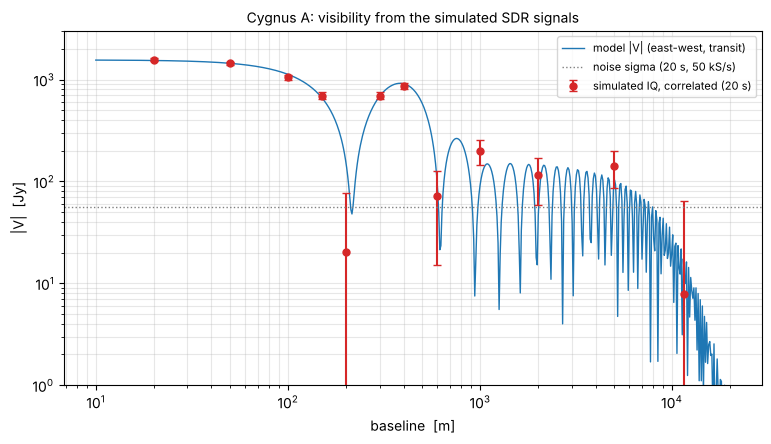
\includegraphics[width=0.9\textwidth]{images/signal_check.png}
  \caption{Cygnus~A at 1420\,MHz: visibility amplitude of the sky model
           (line) and correlated simulated IQ streams of two 3\,m dishes
           with the B210, 20\,s at 50\,kS/s (points with $1\sigma$ error
           bars). Notebook \texttt{03\_signal\_simulation.ipynb}, section~4.}
  \label{fig:signal-check}
\end{figure}

\section{Baseband and quantisation}
\label{sec:baseband}
\index{complex baseband}\index{IQ imbalance}\index{quantisation efficiency}

Module \texttt{signal.baseband} (version~0.9.2, theory notebook
\texttt{C\_sampling\_iq.ipynb}) describes the imperfections of the receive
path between the antenna and the samples:

\begin{description}
  \item[\texttt{iq\_imbalance}, \texttt{image\_rejection\_db}] gain error $g$
        and phase error $\varphi$ between the I and Q branches; a tone at $+f$
        gets an image at $-f$, suppressed by
        $\mathrm{IRR} = (1+2g\cos\varphi+g^2)/(1-2g\cos\varphi+g^2)$
        (0.1\,dB and $1^\circ$: 40\,dB; 0.5\,dB and $3^\circ$: 28\,dB). A DC offset
        (LO leakage) common to the two channels of one B210 correlates in the
        centre channel and is flagged; the automatic corrections of the B210
        stay off.
  \item[\texttt{quantizer\_levels}, \texttt{quantization\_efficiency}] thresholds
        and levels of the mid-rise quantiser of \texttt{quantize} and its
        efficiency for weak correlations,
        $\eta_Q = [\sum_k y_k(\phi(t_k)-\phi(t_{k+1}))]^2 /
        \sum_k y_k^2(\Phi(t_{k+1})-\Phi(t_k))$: 0.637 (1 bit), 0.881 (2 bits),
        0.963 (3 bits), 0.989 (4 bits) at the optimum steps; measured with
        \texttt{quantize} 0.624, 0.877, 0.960, 0.988 (statistical error 0.014).
  \item[\texttt{van\_vleck\_1bit}] the arcsine law
        $\rho_q = \frac{2}{\pi}\arcsin\rho$ and its inverse.
\end{description}
2 bits keep 88\,\% of the correlation with a quarter of the data volume of
8 bits; two B210 channels at 2\,MS/s need 58\,GB/h in \texttt{sc16}, 7.2\,GB/h
re-quantised to 2 bits (Fig.~\ref{fig:iq-quant}). The usable band is the inner
$\approx 80\,\%$ of the channels (anti-aliasing filter, Fig.~\ref{fig:iq-edges}).

\begin{figure}[htbp]
  \centering
  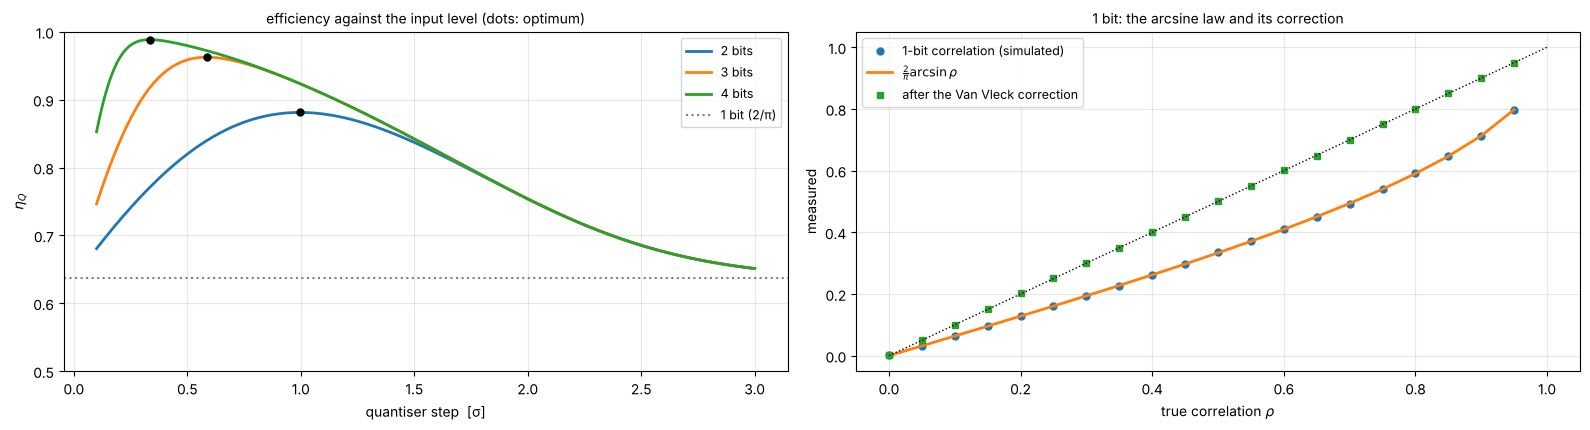
\includegraphics[width=\textwidth]{images/iq_quantisation.png}
  \caption{Quantisation efficiency against the quantiser step (dots: the
           optimum steps of \texttt{quantize}); 1-bit correlation against the
           true one with the arcsine law and the Van Vleck correction.}
  \label{fig:iq-quant}
\end{figure}

\begin{figure}[htbp]
  \centering
  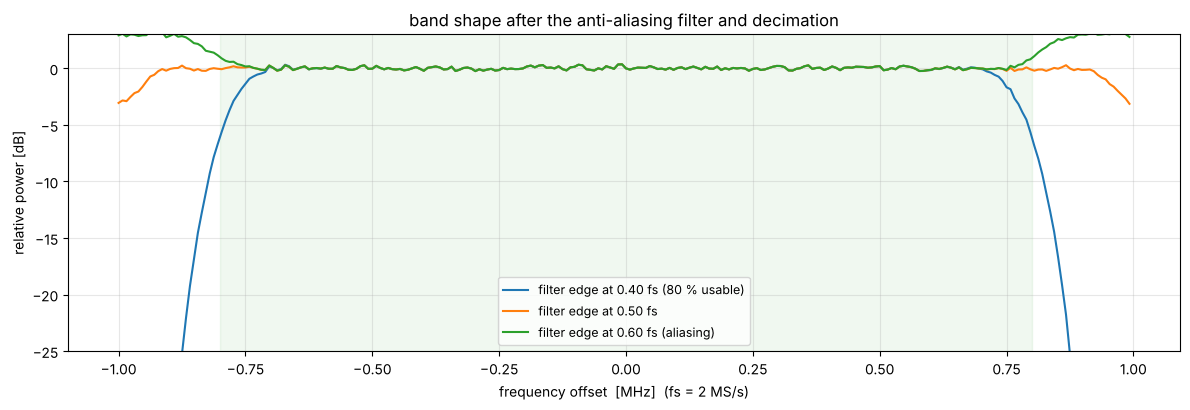
\includegraphics[width=0.8\textwidth]{images/iq_band_edges.png}
  \caption{Band shape after an anti-aliasing filter and decimation to 2\,MS/s
           for three filter edges; shaded: the inner 80\,\% of the band.}
  \label{fig:iq-edges}
\end{figure}
